\documentclass[submission]{eptcs}
\providecommand{\event}{TTC 2014} % Name of the event you are submitting to

\usepackage[usenames,dvipsnames,table]{xcolor}
\usepackage[T1]{fontenc}
\usepackage{geometry}
\usepackage{paralist}
\usepackage{graphicx}
\usepackage[cache]{minted}
\usepackage{url}
\usepackage[utf8]{inputenc}
\usepackage{paralist}
\usepackage{amstext}
\usepackage{amsfonts}
\usepackage{xspace}
\usepackage{todonotes}
\usepackage{hyperref}

\usepackage[skip=0pt]{caption}
\usepackage{setspace}
\setstretch{0.96}

\hypersetup{
  colorlinks, 
  breaklinks, 
  bookmarksnumbered=true,
  pdftitle={Solving the TTC'14 FIXML Case Study with SIGMA},
  pdfauthor={Filip Krikava and Philippe Collet}, 
  linkcolor=Blue, 
  citecolor=BrickRed, 
  filecolor=Blue, 
  urlcolor=Blue
  }

\renewcommand{\ttdefault}{pcr}

\newcommand{\SIGMA}{\textsc{Sigma}\xspace}
\newcommand{\FIXML}{FIXML\xspace}
\newcommand{\TTC}{TTC'14\xspace}
\newcommand{\Csharp}{C\#\xspace}
\newcommand{\Ie}{\emph{i.e.}\xspace}
\newcommand{\Eg}{\emph{e.g.}\xspace}
\newcommand{\Etal}{\emph{et al.}\xspace}
\newcommand{\Cf}{\emph{cf.}\xspace}

\newcommand{\Todo}[1]{\todo[inline]{#1}}
\renewcommand{\Todo}[1]{}

\newminted{scala}{fontsize=\fontsize{8}{8},linenos,numbersep=5pt,frame=lines,framesep=2mm}
\newminted{xml}{fontsize=\fontsize{8}{8},linenos,numbersep=5pt,frame=lines,framesep=2mm}
\newminted{java}{fontsize=\fontsize{8}{8},linenos,numbersep=5pt,frame=lines,framesep=2mm}
\newminted{c}{fontsize=\fontsize{8}{8},linenos,numbersep=5pt,frame=lines,framesep=2mm}
\newmintinline{xml}{fontsize=\fontsize{8}{8}}
\newmintinline{scala}{fontsize=\fontsize{8}{8}}
\newmintinline{c}{fontsize=\fontsize{8}{8}}

\newcommand{\Scala}{\scalainline}

\title{Solving the \TTC \FIXML Case Study with SIGMA}

\author{
  Filip Křikava
  \institute{University Lille 1 - LIFL, France}
  \institute{INRIA Lille, Nord Europe}
  \email{\href{mailto:filip.krikava@inria.fr}{filip.krikava@inria.fr}}
\and
  Philippe Collet
  \institute{Université Nice - Sophia Antipolis, France}
  \institute{CNRS, I3S, UMR 7271}
  \email{\quad \href{mailto:philippe.collet@unice.fr}{philippe.collet@unice.fr}}
}

\def\titlerunning{Solving the \TTC \FIXML Case Study with SIGMA}
\def\authorrunning{F. Křikava and P. Collet}

\begin{document}
\maketitle

\begin{abstract}
In this paper we describe a solution for the \emph{Transformation Tool Contest 2014} (\TTC) FIXML case study using \SIGMA, a family of Scala internal \emph{Domain-Specific Languages} (DSLs) for model manipulation that provides expressive and efficient API for model consistency checking and model transformations.
The solution solves the core transformation task as well as all the three extensions.
\end{abstract}

%!TEX root = ttc14-fixml.tex

\section{Introduction}
\label{sec:Introduction}

%% Overview
In this paper we describe the solution for the \TTC \FIXML case study~\cite{Lano2014} using the \SIGMA internal DSLs~\cite{Krikava2014}.
The case study involves \emph{text-to-model} (T2M), \emph{model-to-model} (M2M) and \emph{model-to-text} (M2T) transformations, generating Java, \Csharp, C++ code from a \FIXML XML messages.
Furthermore, we describe our approach to the three proposed extensions.
The complete solution is available on a Github\footnote{\url{https://github.com/fikovnik/ttc14-fixml-sigma}} as well as in the SHARE\footnote{\url{http://is.ieis.tue.nl/staff/pvgorp/share/}} environment in the virtual machine image \texttt{Ubuntu12LTS\_TTC14\_64bit\_SIGMA.vdi}.

%% SIGMA
The solution is developed in \SIGMA, a family of Scala\footnote{\url{http://scala-lang.org/}} internal DSLs for model manipulation tasks such as model validation and model transformations.
Developed as an open source project hosted on Github~\footnote{\url{https://fikovnik.github.io/Sigma}},
\SIGMA is a library that provides a dedicated Scala API allowing to manipulate models using high-level constructs similar to ones found in the external model manipulation DSLs such as ETL~\cite{Kolovos2008a} or ATL~\cite{Jouault2006}.
The intent is to provide an approach that developers can use to implement many of the practical model manipulations within a familiar environment, reduced learning overhead and improved usability.

The solution uses the \emph{Eclipse Modeling Framework} (EMF)~\cite{EMF}, which is a popular meta-modeling framework widely used in both academia and industry.
It is directly supported by \SIGMA, however, other meta-modeling frameworks could be used as well, since \SIGMA transformations are technologically agnostic.

%% Organization
The remainder of this document is organized as follows:
\begin{inparaitem}[]
	\item Section~\ref{sec:SigmaOverview} gives a brief overview of \SIGMA.
	\item Section~\ref{sec:SolutionDescription} describes the solution for the case study core problem.
	\item Section~\ref{sec:Extensions} presents the solutions for the three case study extensions.
	\item Section~\ref{sec:Evaluation} evaluates the solution using the evaluation criteria proposed in the case study, and finally Section~\ref{sec:Conclusion} concludes the paper.
\end{inparaitem}
%
% Additionally, two appendixes are provided.
% \begin{inparaitem}[]
% 	\item Appendix~\ref{sec:Configuration} describes the configuration of the SHARE environment that has been done in order to run the \SIGMA solution and
% 	\item Appendix~\ref{sec:Example} shows the generated Java, \Csharp, C++ and C code resulting from running the solution for the example \texttt{test2.xml} \FIXML message.
% \end{inparaitem}
%!TEX root = ttc14-fixml.tex

\section{Solution Description}
\label{sec:SolutionDescription}

This section describes the solution for the core problem of transforming \FIXML messages into Java, \Csharp and C++ source code.
As suggested, the solution is realized by systematic model transformations that are broken in the following tasks:
\begin{inparaenum}[(1)]
  \item XML text to XML model (T2M transformation),
  \item XML model to a model of an object oriented language (ObjLang) (M2M transformation), and
  \item ObjLang model to source code (M2T transformation).
\end{inparaenum}

\subsection{Overview}

The input for the transformation chain is a file representing an \FIXML message in the \FIXML 4.4 version defined by the \FIXML XML Schema~\cite{FIXML2004}.
The output is the corresponding Java, \Csharp and C++ source codes that represent the data of the given \FIXML message. 
The source concerning the solution to the core problem is located in the \href{https://github.com/fikovnik/ttc14-fixml-sigma/tree/master/ttc14-fixml-base}{\texttt{ttc14-fixml-base}} directory.

\subsection{\FIXML XML Message to XML Model (T2M)}

The T2M transformation consists in parsing an \FIXML XML document and creating an XML that conforms to the XML meta-model as specified in the case study description~\cite{Lano2014} (\Cf Figure~\ref{fig:XMLMetaModel}).

\begin{figure}[h!bt]
  \centering
  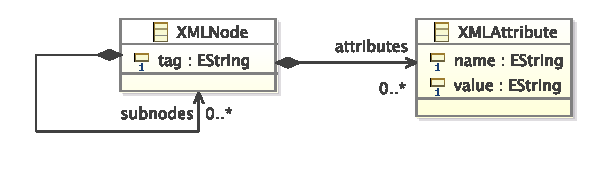
\includegraphics[width=.6\textwidth]{figures/XMLMetaModel.pdf}
  \caption{XML meta-model}
  \label{fig:XMLMetaModel}
\end{figure}

\paragraph{Common Infrastructure.} 
%
The first step before any \SIGMA model manipulation task is to create the common infrastructure for the given model \Ie generate support classes that allows for seamless model navigation and modification using standard Scala expressions.
In the case of EMF models, the common infrastructure aligns EMF generated Java classes with Scala.
This involves
%
\begin{inparaitem}[]
  \item model navigation without \emph{``get noise''} (\Eg \Scala|node.getSubnodes| becomes \Scala|node.subnodes|),
  \item promoting EMF collections to corresponding Scala variants to benefit from convenient first-order logic operations (\Eg, map, filter, reduce), and
  \item first class constructs for creating and initializing new model elements.
\end{inparaitem}

This is addressed by generating extension traits that make EMF model elements interoperable with Scala.
These traits implicitly extend all model classes with property accessors without the \Scala|get| prefix and convert EMF collections into the corresponding Scala ones.
The conversion only happens at the interface level leaving the underlying data storage unchanged.
In the same way, existing Scala types are extended with missing operations (\Eg \Scala|implies|).
For example, the following is an excerpt\footnote{XML meta-model generated code is in the \href{https://github.com/fikovnik/ttc14-fixml-sigma/tree/master/ttc14-fixml-base/src-gen/fr/inria/spirals/sigma/ttc14/fixml/xmlmm/support}{\Scala|fr.inria.spirals.sigma.ttc14.fixml.xmlmm.support|} package.} of the trait generated for the XML meta-model: 
%
\begin{scalacode}
trait XMLMM extends EMFScalaSupport { 
  implicit class XMLNode2Sigma(that: XMLNode) {
    def tag: String = that.getTag
    def tag_=(value: String): Unit = that.setTag(value)
    def subnodes: EList[XMLNode] = that.getSubnodes
    def attributes: EList[XMLAttribute] = that.getAttributes
  }
}
\end{scalacode}
%
Furthermore, for each class in the meta-model, a Scala trait is generated that allows one to create the class instances in a concise way and also allows the classes to participate in Scala pattern matching constructs.

The \href{https://github.com/fikovnik/ttc14-fixml-sigma/blob/master/ttc14-fixml-base/src/fr/inria/spirals/sigma/ttc14/fixml/support/GenerateModelSupport.scala}{\Scala|GenerateModelSupport|} class is responsible for generating the common infrastructure for the EMF models used in this solution.
It is a Scala executable object that first launches the standard EMF code generator to generate Ecore Java classes which is followed by the \SIGMA common infrastructure generator.
It is done in the way that the resulting sources go into the \Scala{src-gen} directory instead of the \Scala{src}, so that the generated code is separated from the user written one.
This class has to be re-run every time any of the models changes.

\paragraph{Transformation.}
%
With the above model navigation and manipulation support, we can implement the actual transformation.
Parsing XML is a common task and Scala already provides a solid support that is built into the language (\Eg XML literals).
The object \href{https://github.com/fikovnik/ttc14-fixml-sigma/blob/master/ttc14-fixml-base/src/fr/inria/spirals/sigma/ttc14/fixml/FIXMLParser.scala}{\Scala|FIXMLParser|} is responsible for the transformation.
It tries to parse FIXML message coming from various inputs (\Eg, text, file, input stream) and build the corresponding XML model.
The actual transformation happens in the \Scala|parseNodes| and \Scala|parseAttributes| methods:

\begin{scalacode}
protected def parseNodes(nodes: Iterable[Node]): Iterable[XMLNode] = {
  val elems = nodes collect { case e: Elem => e }

  for (elem <- elems) yield XMLNode(
    tag = elem.label,
    subnodes = parseNodes(elem.child),
    attributes = parseAttributes(elem.attributes))
}

protected def parseAttributes(metaData: MetaData) =
  metaData collect {
    case e: xml.Attribute => XMLAttribute(name = e.key, value = e.value.toString)
  }
\end{scalacode}

On the line 2 we discard any potential PCDATA nodes (\Eg white spaces) and then we simply yield a new \Scala|XMLNode| for \Scala|xml.Node| that has been parsed from XML.
Only well-formed documents are considered since the underlying Scala XML library throws parsing exception in cases the input document is not well-formed.
Additionally, we check for the presence of \xmlinline|<FIXML>| tag and provide a simple mechanism to discard \FIXML messages that are not in the desired \FIXML 4.4 Schema version.

\subsection{XML Model to ObjLang Model (M2M)}

This task involves transforming the XML model created in the previous section into a model of an object oriented language, ObjLang.

\paragraph{ObjLang meta-model.}
%
The meta-model of the ObjLang model used in this solution is shown in Figure~\ref{fig:ObjLangMetaModel}.
%
\begin{figure}[h!bt]
  \centering
  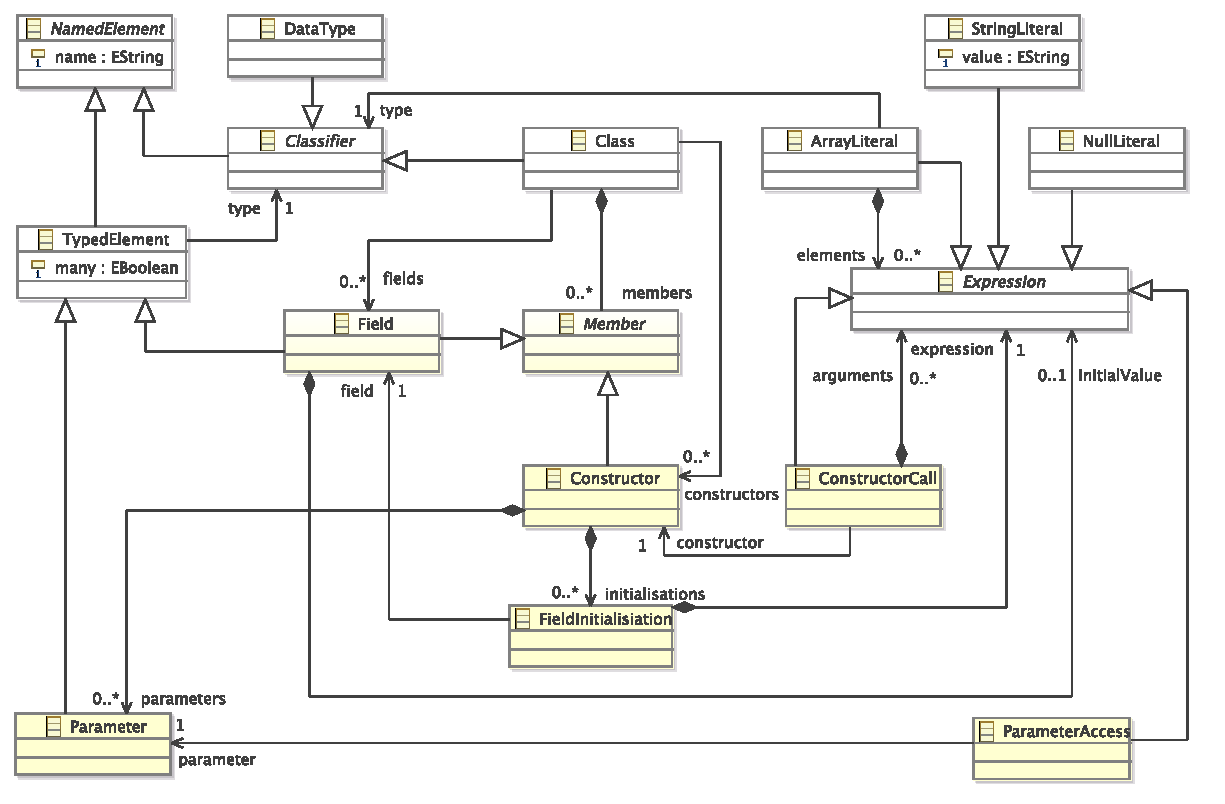
\includegraphics[width=\textwidth]{figures/ObjLangMetaModel.pdf}
  \caption{ObjLang meta-model}
  \label{fig:ObjLangMetaModel}
\end{figure}
%
It originates from the Featherweight Java model~\cite{Igarashi2001}, concretely from the version available at the EMFtext website\footnote{\url{http://www.emftext.org/index.php/EMFText_Concrete_Syntax_Zoo_Featherweight_Java}}.
It provides a reasonable abstraction over the close yet different models of the concerned programming languages.
The model supports basic classes with fields, data types that are organized in a similar fashion as in Ecore (\Ie separating external types from model classes), and a basic set of expressions that is used for field initializations.
The model itself more closely resembles a Java model than for example a C++ model.
For example, a \Scala|Field| can optionally have an initial value, which is a feature not supported in C++\footnote{Initial values of fields in C++ are set in a constructor initializer list or in its body.}.
These differences are left to be handled by the M2T transformers since the aim is to have just a single language agnostic meta-model.

\paragraph{Transformation.}
%
An M2M transformation provides necessary support for translating models into other models, essentially by mapping source model elements into corresponding target model elements.
An imperative style of M2M transformation~\cite{Czarnecki2006} is already supported thanks to the common infrastructure layer described above.
On the other hand, the lower level of abstraction of the imperative transformation style leaves users to manually address issues such as orchestrating the transformation execution and resolving target elements against their source counterparts~\cite{Kolovos2008a}.
Therefore, inspired by ETL and ATL, we provide a dedicated internal DSL that combines the imperative features with declarative rule-based execution scheme into a hybrid M2M transformation language.

In \SIGMA a M2M transformation is represented as a Scala class that inherits from the \Scala|M2MT| base class, which itself brings M2M DSL constructs into the class scope.
Concretely, the \href{https://github.com/fikovnik/ttc14-fixml-sigma/blob/master/ttc14-fixml-base/src/fr/inria/spirals/sigma/ttc14/fixml/XMLMM2ObjLang.scala}{\Scala|XMLMM2ObjLang|} class is defined as:
%
\begin{scalacode}
class XMLMM2ObjLang extends M2MT with XMLMM with ObjLang {

  sourceMetaModels = _xmlmm
  targetMetaModels = _objlang

  // transformation rules
}  
\end{scalacode}
%
Next to extending from the \Scala|M2MT| base class, it also mixes the \Scala|XMLMM| and \Scala|ObjLang| traits which are the generated support for the respective models participating in this transformation.
In lines 3 and 4 it further specifies the transformation source and target models.
In this case we translate one model into another one, but multiple models are supported.

The transformation rules are specified as methods.
For example, the first rule of the transformation is defined as:
%
\begin{scalacode}
def ruleXMLNode2Class(s: XMLNode, t: Class) {
  s.allSameSiblings foreach (associate(_, t))

  t.name = s.tag
  t.members ++= s.sTargets[Constructor]
  t.members ++= s.allAttributes.sTarget[Field]
  t.members ++= s.allSubnodes.sTarget[Field]
}
\end{scalacode}

This method creates a rule named \Scala|XMLNode2Class| that transforms an \Scala|XMLNode| into a \Scala|Class|.
A transformation rule in \SIGMA may optionally define additional targets, but there is always one primary source to the target relation.
This rule represents a matched rule which is automatically applied for all matching elements.
When such a rule is executed, the transformation engine first creates all the defined target elements and then calls the method whose body populates their content using arbitrary Scala code.
Inside the method body, additional target elements can be constructed (using the support provided by the common infrastructure), but in such a case, the developer is responsible for their proper containment and there will be no trace links associated with them.

A matched rule is applied once and only once for each matching source element, creating a 1:1 or 1:N mapping.
However, this is not the case in the current scenario where XML document may contain multiple sibling elements with the same tag name which all should be mapped into an exact same class.
This is done by associating all the same-tag siblings to the very same class during the rule application on the first of them (line 2).
The method \Scala|allSameSiblings| is a helper method that collects all the elements that have the same tag and are at the same level.

The next four lines (4-7) populates the content of the class.
The expression on the line 5 \Scala|t.members ++= s.sTargets[Constructor]| assigns all constructors that can be transformed from the source XML node into the class.
Similarly \Scala|t.members ++= s.allAttributes.sTarget[Field]| add fields that have been transformed from the XML node attributes.
The two methods \Scala|sTarget| and \Scala|sTargets| are defined on all model elements.
They provide a way to relate the corresponding target elements that have been already or can be transformed from source elements.
The difference between them is that \Scala|sTarget| should be used in the case of 1:N relationship between the source and target as opposed to 1:1 in the case of \Scala|sTarget|.

As for constructors, they are transformed using the following two rules:
%
\begin{scalacode}
def ruleXMLNode2DefaultConstructor(s: XMLNode, t: Constructor) {
  s.allSameSiblings foreach (associate(_, t))
}

def ruleXMLNode2NonDefaultConstructor(s: XMLNode, t: Constructor) = guardedBy {
  !s.isEmptyLeaf
} transform {

  s.allSameSiblings foreach (associate(_, t))

  for (e <- (s.allAttributes ++ s.allSubnodes.distinctBy(_.tag))) {
    val param = e.sTarget[Parameter]
    val field = e.sTarget[Field]

    t.parameters += param
    t.initialisations += FieldInitialisiation(
      field = field,
      expression = ParameterAccess(parameter = param))
  }
}
\end{scalacode}
%
The first one denotes a default (zero-argument) constructor.
As we have discussed earlier, the ObjLang favors field initialization to constructor initialization and therefore the rule body is almost empty.
The single expression is the very same association that ensures that all same-tag sibling nodes maps to the same default constructor.

Unlike the default constructor, the rule creating a non-default constructor should only be applicable in the case there is at least one field to be set.
In \SIGMA this condition is represented by a rule guard that can further limit rule application using a boolean expression.
The \Scala|!s.isEmptyLeaf| checks whether there is at least one attribute or a subnode in any of the same-tag siblings.
It then creates a constructor parameter for each of the attributes and subnodes and uses them to initialize the class fields.

The constructor parameters are created using the following two rules, one for XML attribute and one for XML node.
The \Scala|@LazyUnique| annotation denotes a lazy unique rule.
Such rule is not automatically applied for matching elements and instead it has to be explicitly called using the \Scala|sTarget| or \Scala|sTargets| methods.
Unlike lazy rule (annotated by \Scala|@Lazy|), it establishes a transformation trace between the source and targets and therefore it always returns the same targets for a given source.
%
\begin{scalacode}
@LazyUnique
def ruleXMLAttribute2ConstructorParameter(s: XMLAttribute, t: Parameter) {
  t.name = checkName(s.name)
  t.type_ = s.sTarget[Field].type_
}

@LazyUnique
def ruleXMLNode2ConstructorParameter(s: XMLNode, t: Parameter) {
  val field = s.sTarget[Field]

  t.name = field.name
  t.many = field.many
  t.type_ = field.type_
}
\end{scalacode}

The class fields are populated from the \Scala|ruleXMLNode2Class| rule (lines 6 and 7).
It calls the following two lazy unique rules:
%
\begin{scalacode}
@LazyUnique
def ruleXMLAttribute2Field(s: XMLAttribute, t: Field) {
  t.name = checkName(s.name)

  t.type_ = DTString
  t.initialValue = StringLiteral(s.value)
}

@LazyUnique
def ruleXMLNode2Field(s: XMLNode, t: Field) {
  val allSiblings = s.allSameSiblings
  allSiblings foreach (associate(_, t))

  t.type_ = s.sTarget[Class]

  val groups = (s +: allSiblings) groupBy (_.eContainer)
  val max = groups.values map (_.size) max

  if (max > 1) {
    t.name = s.tag + "_objects"
    t.many = true
    val init = ArrayLiteral(type_ = s.sTarget[Class])
    val siblings = groups(s.eContainer)
    
    init.elements ++= siblings.sTarget[ConstructorCall]
    init.elements ++= 0 until (max - siblings.size) map (_ => NullLiteral())
    t.initialValue = init
  } else {
    t.name = s.tag + "_object"
    t.initialValue = s.sTarget[ConstructorCall]
  }
}  
\end{scalacode}
%
The first one translates an XML attribute into a field.
In the core problem specification, only string data types are used and therefore it assigns string data type regardless of the actual value of the attribute.
In order not to conflict with language programming keywords, we provide a check that simply prepends the name with an underscore.
The name conflicts could also be handled later at the M2T level, where each transformer can include a list of its language keywords.
However, this could result in a state in which different names would be used for the same fields making the code inconsistent.

The second rule converts an XML node into a field.
It has to handle the case of having a multiple same-tag siblings.
The case description proposes to use either multiple fields initialized by specific constructors or by an array/list of such objects.
While the former is easier to implement (simply by making the rule lazy), it creates a scalability problem since in Java, there is a limit of the maximum number of method parameters.
For example the test case \texttt{test5.xml} already exceeds this number.
Therefore we have opted for the latter solution and use arrays to represent multiple same-tag sibling nodes.
The number of same-tag sibling nodes can vary within a parent node.
For example:
%
\inputminted[fontsize=\fontsize{8}{8},linenos,numbersep=5pt,frame=lines,framesep=2mm]{xml}{listings/variable-siblings.xml}
%
The \Scala|Sub| should be represented by an array field and the default initialization of \Scala|PosRpt| should equal to the following (in Java):
\begin{javacode}
public Pty[] Pty_objects = new Pty[] { 
  new Pty("OCC", "21", null, new Sub[] { null, null }),
  new Pty("C", "38", null, new Sub[] { new Sub("ZZZ", "2", null), null }),
  new Pty("C", "38", "Q", new Sub[] { new Sub("ZZZ", "2", null), new Sub("ZZZ", "3", "X") }) 
};
\end{javacode}
Note that the first and second instances of \Scala|Pty| contains two and one \Scala|null| respectively in the place of missing \Scala|Sub| subnode.

The \Scala|ConstructorCall| used for field initializations in the \Scala|ruleXMLNode2Field| is created from an XML node using the last rule in the transformation:
%
\begin{scalacode}
@Lazy
def ruleXMLNode2ConstructorCall(s: XMLNode, t: ConstructorCall) {
  val constructor = s.sTargets[Constructor]
    .find { c =>
      (c.parameters.isEmpty && s.isEmptyLeaf) ||
      (c.parameters.nonEmpty && !s.isEmptyLeaf)
    }
    .get

  t.constructor = constructor

  t.arguments ++= {
    for {
      param <- constructor.parameters
      source = param.sSource.get
    } yield {
      source match {
        case attr: XMLAttribute =>
          // we can cast since attributes have always primitive types
          val dataType = param.type_.asInstanceOf[DataType]

          s.attributes
            .find(_.name == attr.name)
            .map { local => StringLiteral(local.value) }
            .getOrElse(NullLiteral())

        case node: XMLNode =>
          s.subnodes.filter(_.tag == node.tag) match {

            case Seq() if !param.many =>
              NullLiteral()
            case Seq(x) if !param.many =>
              x.sTarget[ConstructorCall]
            case Seq(xs @ _*) =>
              val groups = (node +: node.allSameSiblings) groupBy (_.eContainer)
              val max = groups.values map (_.size) max
              
              val init = ArrayLiteral(type_ = param.type_)
              init.elements ++= xs.sTarget[ConstructorCall]
              init.elements ++= 0 until (max - xs.size) map (_ => NullLiteral())
              init
          }
      }
    }
  }
}
\end{scalacode}  

First we need to find which constructor shall be used depending whether the given XML node (or any of its same-tag siblings) contains any attributes or subnodes.
Next, we need to resolve the arguments for the case of non-default constructor.
We do this by using the sources, \Ie, the source elements (XML node or XML attribute) that were used to create the constructor parameters.
\SIGMA provides \Scala|sSource| method that is the inverse of \Scala|sTarget| call with the difference that it will not trigger any rule execution.
In the pattern matching we need to cover all possible cases such as an attribute defined locally or an attribute defined in a same-tag sibling, thus using \Scala|null| for its initialization.

\subsection{ObjLang Model to Source code (M2T)}

This task involves transforming the ObjLang model into source code for various programming languages.
In the core problem solution, Java, \Csharp and C++ are considered.

M2T transformations translate models into text by mapping source model elements into corresponding textual fragments.
\SIGMA provides a template-based approach whereby string patterns are extended with executable logic for code selection and iterative expansion~\cite{Czarnecki2006}.
Unlike most of the external DSLs for M2T transformation, \SIGMA uses the code-explicit form, \Ie, it is the output text instead of the transformation code that is escaped.
From our experience, in non-trivial code generations, the quantity of text producing logic usually outweighs the text being produced.
For the parts where there is more text than logic we rely on Scala multi-line string literals and string interpolations allowing one to embed variable references and expressions directly into strings.

Since we target multiple programming languages at the same time, we organize the code generation in a set of Scala classes and rely on Scala class inheritance and class mix-ins to compose, in a modular way, configuration for the respective languages.
In the base class \href{https://github.com/fikovnik/ttc14-fixml-sigma/blob/master/ttc14-fixml-base/src/fr/inria/spirals/sigma/ttc14/fixml/BaseObjLangMTT.scala}{\Scala{BaseObjLangMTT}} we define methods that synthesize expressions and data types.
The default (Java) implementation can be then easily overwritten by other languages.
Next we abstract a class generation into \href{https://github.com/fikovnik/ttc14-fixml-sigma/blob/master/ttc14-fixml-base/src/fr/inria/spirals/sigma/ttc14/fixml/BaseObjLang2Class.scala}{\Scala{BaseObjLang2Class}}.
The code generation is split into a fine-grained templates, represented as regular Scala methods, that generates fields, constructors and the like:
%
\begin{scalacode}
abstract class BaseObjLang2Class extends BaseObjLangMTT {

  type Source = Class

  def main = {
    header
    
    !s"class ${source.name}" curlyIndent {
      genFields

      !endl

      genConstructors
    }
    
    footer
  }
  
  def genConstructors =
    source.constructors foreach genConstructor

  def genFields =
    source.fields foreach genField

  def genField(c: Field) =
    !s"public ${type2Code(c)} ${c.name}${toInitCode(c)};"

  def toInitCode(f: Field) = 
    " = " + (f.initialValue map toCode getOrElse (""))
    
  def genConstructor(c: Constructor) = {
    val args = c.parameters map param2Code mkString (", ")

    !s"public ${source.name}($args)" curlyIndent {
      c.initialisations foreach genFieldInitialization
    }

    !endl
  }

  def genFieldInitialization(fi: FieldInitialisiation) =
    !s"this.${fi.field.name} = ${toCode(fi.expression)};"
    
}  
\end{scalacode}
%
Together with the \href{https://github.com/fikovnik/ttc14-fixml-sigma/blob/master/ttc14-fixml-base/src/fr/inria/spirals/sigma/ttc14/fixml/ObjLang2Java.scala}{\Scala{ObjLang2Java}} class, a complete ObjLang to Java transformer can be instantiated.
The class \href{https://github.com/fikovnik/ttc14-fixml-sigma/blob/master/ttc14-fixml-base/src/fr/inria/spirals/sigma/ttc14/fixml/ObjLang2Java.scala}{\Scala{ObjLang2Java}} contains the Java language specifics which, in this case, is only the name of the \Scala{string} data type.
%
\begin{scalacode}
trait ObjLang2Java extends BaseObjLangMTT {
  override def class2Code(p: DataType) = "String"
}
\end{scalacode}

The generator for the \Csharp is exactly the same and the class \href{https://github.com/fikovnik/ttc14-fixml-sigma/blob/master/ttc14-fixml-base/src/fr/inria/spirals/sigma/ttc14/fixml/ObjLang2CSharp.scala}{\Scala{ObjLang2CSharp}} also only defines the \Scala{string} data type.

For C++, the situation is a bit more complicated, since we need to generate two files, a header and an implementation file.
Also the C++ syntax differs from the one of Java a bit more.





% An important aspect of any M2T transformation language is the template readability, \Eg, layout and indentation.
% The internal DSL maintains it through dedicated support for decorators, smart whitespace handling and relaxed newlines.
% Decorators are nestable string operations that reformat a given block.
% For example, on line 4 we use \Codeinline{curlyIndent} decorator, that wraps its body into a pair of curly brackets and indent each line.
% Smart whitespace handler removes extra whitespace from multi-line strings that are there only for the template readability.
% For example the whitespaces prefixing the text on lines 14 and 15 will be discarded.
% Relaxed newlines loosen the necessity to output new line characters by doing it automatically after every text output.
% Both smart whitespace and newlines handlers are enabled by default, but can be turned off.



% %!TEX root = ttc14-fixml.tex

\section{Extensions}
\label{sec:Extensions}

\subsection{Extension 1 - Selection of Appropriate Data Types}
\label{sec:Extension1}

The aim of the first extension is to further refine the data type used by the XML node attributes and use more appropriate type than just a generic string.
The source concerning this is located in the \href{https://github.com/fikovnik/ttc14-fixml-sigma/tree/master/ttc14-fixml-extension-1}{\texttt{ttc14-fixml-extension-1}} directory.

\bigskip

There are three changes needed in order to implement this extension.
\begin{itemize}[(1)]
	\item The first one is in the ObjLang meta-model where we need to add new expression classes representing literals for the new data types.
	In this extension we consider following new data types: \Scala{double}, \Scala{long} and \Scala{integer}.
	While this list does not cover all the possible XML Schema data types, it provides a good base for demonstrating how a support for additional ones could be added.

	\item The second one concerns the M2M transformation.
	We have to add the necessary support for guessing the data type of an attribute based on the string values from all of the same-tag siblings that have have the attribute in question.
	Following is the code snippet that realize it:
	%
	\begin{scalacode}
	  // basic types
	  val DTString = DataType(name = "string")
	  val DTDouble = DataType(name = "double")
	  val DTLong = DataType(name = "long")
	  val DTInteger = DataType(name = "int")

	  // it also stores the promotion ordering from righ to left
	  val Builtins = Seq(DTString, DTDouble, DTLong, DTInteger)

	  private val PDouble = """([+-]?\d+.\d+)""".r
	  private val PInteger = """([+-]?\d+)""".r

	  def guessDataType(value: String): DataType = value match {
	    case PDouble(_) => DTDouble
	    case PInteger(_) => Try(Integer.parseInt(value)) map (_ => DTInteger) getOrElse (DTLong)
	    case _ => DTString
	  }

	  def guessDataType(values: Seq[String]): DataType =
	    values map guessDataType reduce { (a, b) =>
	      if (Builtins.indexOf(a) < Builtins.indexOf(a)) a else b
	    }
	\end{scalacode}

	\item Finally, we need to update the code transformers to generate the appropriate data types.
	For example, in the C++ generator:
	\begin{scalacode}
override def class2Code(p: DataType) = {
  import XMLMM2ObjLang._
  p match {
    case DTString => "std::string"
    case DTDouble => "double"
    case DTLong => "long"
    case DTInteger => "int"
  }
}		
	\end{scalacode}
\end{itemize}

\subsection{Extension 2 - Extension to Additional Languages}
\label{sec:Extension2}

This extension adds a support for the C language.
Since C is not an object oriented language, more work have to be done in the code generator part.
It is important to node, that the M2M or T2M transformations have to remain untouched.

Instead of classes, in the case of the C language, we generate C structs with appropriate functions simulating object constructors.
For each ObjLang class we generate a header file with a struct definition, a function for the struct creation and a set of functions representing class constructors.
Following is an example of the C code synthesized from this \FIXML message (for the \Scala|Pty| node):
%
\inputminted[fontsize=\fontsize{8}{8},linenos,numbersep=5pt,frame=lines,framesep=2mm]{xml}{listings/example-for-c-code.xml}
%
\begin{ccode}
#ifndef _Pty_H_
#define _Pty_H_

#include <stdlib.h>

#include "Sub.h"

typedef struct {
  char* _R;
  char* _ID;
  Sub** Sub_objects;
} Pty;

Pty* Pty_new();
Pty* Pty_init_custom(Pty* this, char* _R, char* _ID, Sub** Sub_objects);
Pty* Pty_init(Pty* this);

#endif // _Pty_H_	
\end{ccode}
%
\begin{ccode}
#include "arrays.h"

#include "Pty.h"

Pty* Pty_new() {
  return (Pty*) malloc(sizeof(Pty));
}
Pty* Pty_init_custom(Pty* this, char* _R, char* _ID, Sub** Sub_objects) {
  this->_R = _R;
  this->_ID = _ID;
  this->Sub_objects = Sub_objects;
  return this;
}

Pty* Pty_init(Pty* this) {
  this->_R = "21";
  this->_ID = "OCC";
  this->Sub_objects = (Sub**) new_array(2, Sub_init_custom(Sub_new(), "2", "ZZZ"), NULL);
  return this;
}
\end{ccode}

In order to simplify the code generator, we use a helper function \cinline{void **new_array(int size, ...)} that allows us to initialize arrays using simple expressions.
Something that is not directly supported by C language or by the standard C library.

The source concerning the extension 2 solution is in the \href{https://github.com/fikovnik/ttc14-fixml-sigma/tree/master/ttc14-fixml-extension-2}{\texttt{ttc14-fixml-extension-2}} directory.

\subsection{Extension 3 - Generic Transformation}
\label{sec:Extension3}

\Todo{Extension 3}


The source concerning the extension 3 solution is in the \href{https://github.com/fikovnik/ttc14-fixml-sigma/tree/master/ttc14-fixml-extension-3}{\texttt{ttc14-fixml-extension-3}} directory.

% %!TEX root = ttc14-fixml.tex
\vspace*{-3mm}
\section{Evaluation and Conclusion}
\label{sec:EvaluationConclusion}

\enlargethispage{7mm}

We evaluate our solution to the core problem using the evaluation criteria proposed in the case study description~\cite{Lano2014}.

\begin{itemize}[-]
  \item The \emph{complexity} as the number of operator occurrences, features and entity type name references in the specification expressions.
  To the best of our knowledge there is no tool providing this metric for Scala code.
  We therefore only provide our own estimate for the M2M transformation, which contains about 450 expressions and uses 18 meta-models classes with 23 references.

  \item The \emph{accuracy} measures the syntactical correctness of the generated source code and how well the code represents the \FIXML messages.
  The generated code compiles for all languages without any warning nor any special compiler settings\footnote{The C/C++ \texttt{-fPIC} option is a standard option allowing the object files to be included in libraries.}.
  Using arrays to represent same-tag sibling nodes improves the quality and scalability of the code which is further enhanced by data type heuristics for field types.
  Finally, we have also implemented the generic \FIXML Schema transformation that should result in a complete representation of \FIXML messages in the different languages.

  \item The development effort is estimated to be about 15 person-hours for the core problem.

  \item The \emph{fault tolerance} is high since the Scala XML library can detect invalid XML with accurate parsing errors.

  \item For all test cases (1, 2, 5 and 6), the \emph{execution time} is about 7500ms for all the transformations on SHARE (\Cf Section~\ref{sec:AppendixExecutionTime}).

  \item \emph{Modularity} for the M2M transformation is $1 - \frac{d}{r} = \frac{7}{8} = 0.125$, where $d$ is the number of dependencies between rules and $r$ is the number of rules.

  \item The level of \emph{abstraction} for both the M2M and M2T transformations is medium since the rules are defined declaratively (high abstraction), but their content is an imperative code (medium).

\end{itemize}

Despite that we opted for a complex ObjLang model, the resulting transformations are rather expressive and quite concise.
The complete implementation of the core problem consists of 500 lines of Scala code\footnote{The extension 1 consists of 550, extension 2 of 720 and extension 3 of 770 source lines of code.}.
This \FIXML case study provides a good illustration for some of the capabilities of an internal DSL approach to model manipulations in the model-driven engineering domain.











\paragraph{Acknowledgment}
This work is partially supported by the Datalyse project \url{www.datalyse.fr}.

\bibliographystyle{eptcs}
\bibliography{references.bib}	

\appendix

%!TEX root = ttc14-fixml.tex

\section{Meta-Models}
\label{sec:MetaModels}

\enlargethispage{20mm}

\subsection{XML Meta-Model}

The XML model specified in the case study description~\cite{Lano2014}.

\begin{figure}[h!bt]
  \centering
  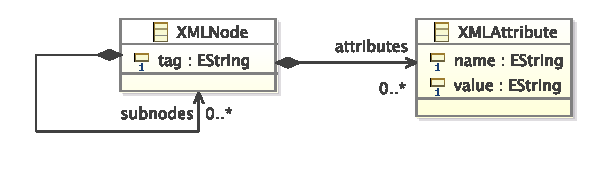
\includegraphics[width=.6\textwidth]{figures/XMLMetaModel.pdf}
  \caption{XML meta-model}
  \label{fig:XMLMetaModel}
\end{figure}

\subsection{ObjLang Meta-Model}

The meta-model representing an object oriented language originating from the Featherweight Java model~\cite{Igarashi2001} (concretely from the version available at the EMFtext website\footnote{\url{http://www.emftext.org/index.php/EMFText_Concrete_Syntax_Zoo_Featherweight_Java}}).

\begin{figure}[h!bt]
  \centering
  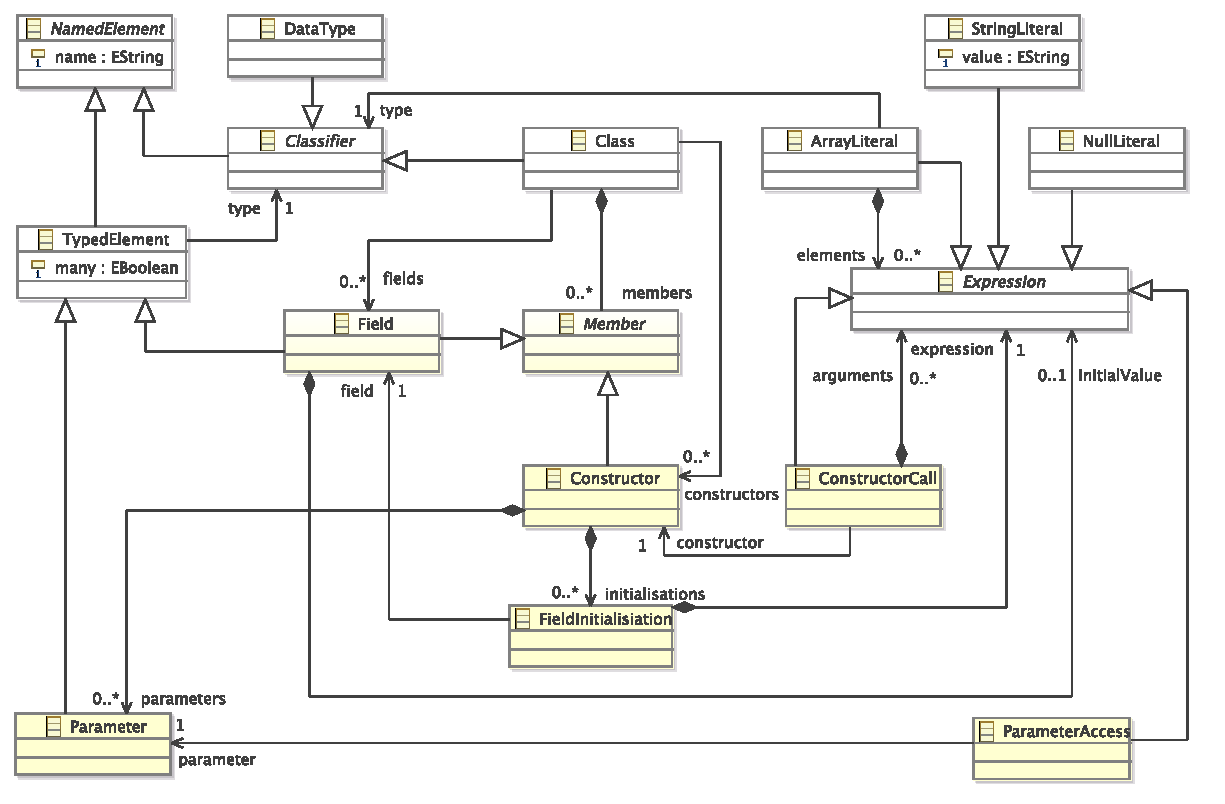
\includegraphics[width=\textwidth]{figures/ObjLangMetaModel.pdf}
  \caption{ObjLang meta-model}
  \label{fig:ObjLangMetaModel}
\end{figure}


%!TEX root = ttc14-fixml.tex

\section{Listings}

\subsection{XML File to XML Model Transformation}
\label{sec:XMLTransfromation}

\subsection{Transformation Rules}
\label{sec:TransformationRules}

\begin{scalacode}
def ruleXMLNode2DefaultConstructor(s: XMLNode, t: Constructor) {
  s.allSameSiblings foreach (associate(_, t))
}
\end{scalacode}

\begin{scalacode}
def ruleXMLNode2NonDefaultConstructor(s: XMLNode, t: Constructor) = guardedBy {
  !s.isEmptyLeaf
} transform {

  s.allSameSiblings foreach (associate(_, t))

  for (e <- (s.allAttributes ++ s.allSubnodes.distinctBy(_.tag))) {
    val param = e.sTarget[Parameter]
    val field = e.sTarget[Field]

    t.parameters += param
    t.initialisations += FieldInitialisiation(
      field = field,
      expression = ParameterAccess(parameter = param))
  }
}
\end{scalacode}

\begin{scalacode}
def ruleXMLAttribute2ConstructorParameter(s: XMLAttribute, t: Parameter) {
  t.name = checkName(s.name)
  t.type_ = s.sTarget[Field].type_
}
\end{scalacode}

\begin{scalacode}
def ruleXMLNode2ConstructorParameter(s: XMLNode, t: Parameter) {
  val field = s.sTarget[Field]

  t.name = field.name
  t.many = field.many
  t.type_ = field.type_
}
\end{scalacode}

\begin{scalacode}
@LazyUnique
def ruleXMLAttribute2Field(s: XMLAttribute, t: Field) {
  t.name = checkName(s.name)

  t.type_ = DTString
  t.initialValue = StringLiteral(s.value)
}
\end{scalacode}

\begin{scalacode}
@LazyUnique
def ruleXMLNode2Field(s: XMLNode, t: Field) {
  val allSiblings = s.allSameSiblings
  allSiblings foreach (associate(_, t))

  t.type_ = s.sTarget[Class]

  val groups = (s +: allSiblings) groupBy (_.eContainer)
  val max = groups.values map (_.size) max

  if (max > 1) {
    t.name = s.tag + "_objects"
    t.many = true
    val init = ArrayLiteral(type_ = s.sTarget[Class])
    val siblings = groups(s.eContainer)
    
    init.elements ++= siblings.sTarget[ConstructorCall]
    init.elements ++= 0 until (max - siblings.size) map (_ => NullLiteral())
    t.initialValue = init
  } else {
    t.name = s.tag + "_object"
    t.initialValue = s.sTarget[ConstructorCall]
  }
}  
\end{scalacode}

\begin{scalacode}
@Lazy
def ruleXMLNode2ConstructorCall(s: XMLNode, t: ConstructorCall) {
  val constructor = s.sTargets[Constructor]
    .find { c =>
      (c.parameters.isEmpty && s.isEmptyLeaf) ||
      (c.parameters.nonEmpty && !s.isEmptyLeaf)
    }
    .get

  t.constructor = constructor

  t.arguments ++= {
    for {
      param <- constructor.parameters
      source = param.sSource.get
    } yield {
      source match {
        case attr: XMLAttribute =>
          // we can cast since attributes have always primitive types
          val dataType = param.type_.asInstanceOf[DataType]

          s.attributes
            .find(_.name == attr.name)
            .map { local => StringLiteral(local.value) }
            .getOrElse(NullLiteral())

        case node: XMLNode =>
          s.subnodes.filter(_.tag == node.tag) match {

            case Seq() if !param.many =>
              NullLiteral()
            case Seq(x) if !param.many =>
              x.sTarget[ConstructorCall]
            case Seq(xs @ _*) =>
              val groups = (node +: node.allSameSiblings) groupBy (_.eContainer)
              val max = groups.values map (_.size) max
              
              val init = ArrayLiteral(type_ = param.type_)
              init.elements ++= xs.sTarget[ConstructorCall]
              init.elements ++= 0 until (max - xs.size) map (_ => NullLiteral())
              init
          }
      }
    }
  }
}
\end{scalacode}
%!TEX root = ttc14-fixml.tex

\section{Handling Constructor Arguments}
\label{sec:ConstructorArguments}

The number of same-tag sibling nodes can vary within a parent node.
For example:

\inputminted[fontsize=\fontsize{8}{8},linenos,numbersep=5pt,frame=lines,framesep=2mm]{xml}{listings/variable-siblings.xml}

The \Scala|Sub| should be represented by an array field and the default initialization of \Scala|PosRpt| should equal to the following (in Java):
%
\begin{javacode}
public Pty[] Pty_objects = new Pty[] { 
  new Pty("OCC", "21", null, new Sub[] { null, null }),
  new Pty("C", "38", null, new Sub[] { new Sub("ZZZ", "2", null), null }),
  new Pty("C", "38", "Q", new Sub[] { new Sub("ZZZ", "2", null), new Sub("ZZZ", "3", "X") }) 
};
\end{javacode}
%
Note that the first and second instances of \Scala|Pty| contains two and one \Scala|null| respectively in the place of missing \Scala|Sub| subnode.

The \Scala|ConstructorCall| used for field initializations in the \Scala|ruleXMLNode2Field| is created from an XML node using the last rule in the transformation:
%
\begin{scalacode}
@Lazy
def ruleXMLNode2ConstructorCall(s: XMLNode, t: ConstructorCall) {
  val constructor = s.sTargets[Constructor]
    .find { c =>
      (c.parameters.isEmpty && s.isEmptyLeaf) ||
      (c.parameters.nonEmpty && !s.isEmptyLeaf)
    }
    .get

  t.constructor = constructor

  t.arguments ++= {
    for {
      param <- constructor.parameters
      source = param.sSource.get
    } yield {
      source match {
        case attr: XMLAttribute =>
          // we can cast since attributes have always primitive types
          val dataType = param.type_.asInstanceOf[DataType]

          s.attributes
            .find(_.name == attr.name)
            .map { local => StringLiteral(local.value) }
            .getOrElse(NullLiteral())

        case node: XMLNode =>
          s.subnodes.filter(_.tag == node.tag) match {

            case Seq() if !param.many =>
              NullLiteral()
            case Seq(x) if !param.many =>
              x.sTarget[ConstructorCall]
            case Seq(xs @ _*) =>
              val groups = (node +: node.allSameSiblings) groupBy (_.eContainer)
              val max = groups.values map (_.size) max
              
              val init = ArrayLiteral(type_ = param.type_)
              init.elements ++= xs.sTarget[ConstructorCall]
              init.elements ++= 0 until (max - xs.size) map (_ => NullLiteral())
              init
          }
      }
    }
  }
}
\end{scalacode}  

First we need to find which constructor shall be used depending whether the given XML node (or any of its same-tag siblings) contains any attributes or subnodes.
Next, we need to resolve the arguments for the case of non-default constructor.
We do this by using the sources, \Ie, the source elements (XML node or XML attribute) that were used to create the constructor parameters.
\SIGMA provides \Scala|sSource| method that is the inverse of \Scala|sTarget| call with the difference that it will not trigger any rule execution.
In the pattern matching we need to cover all possible cases such as an attribute defined locally or an attribute defined in a same-tag sibling, thus using \Scala|null| for its initialization.

%!TEX root = ttc14-fixml.tex

\section{M2T Transformation Class Hierarchy}
\label{sec:M2TClassHierarchy}

\begin{figure}[h!bt]
  \centering
  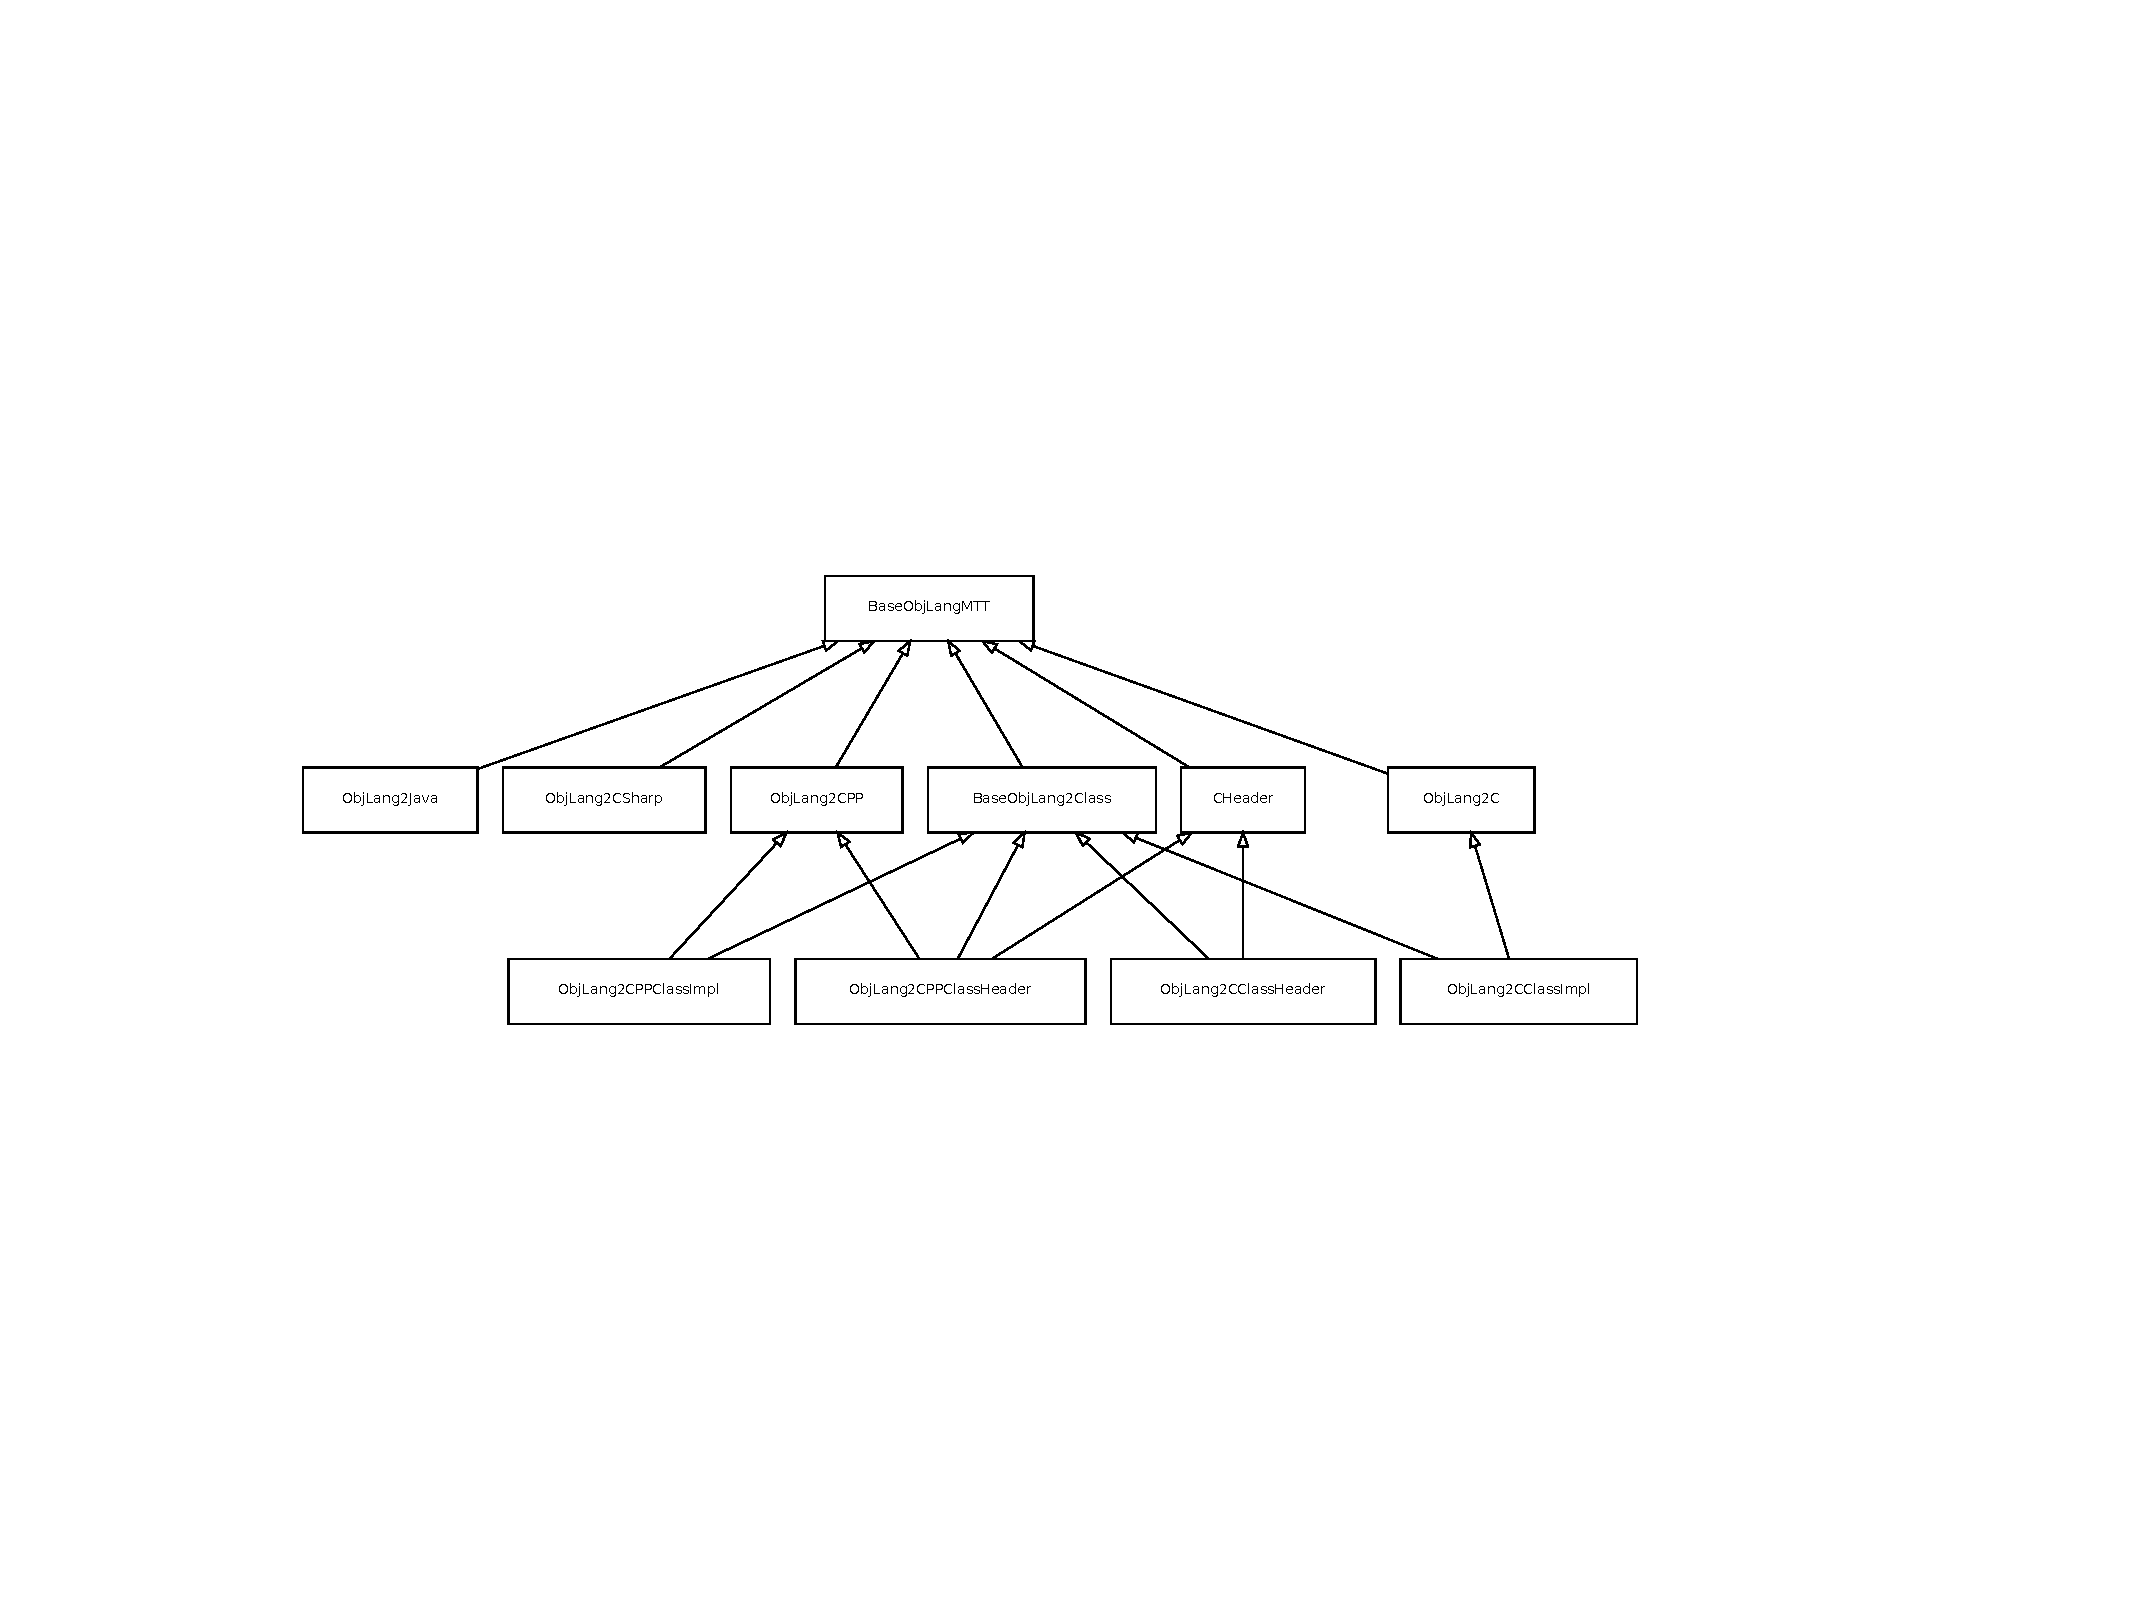
\includegraphics[width=\textwidth]{figures/M2TClassHierarchy.pdf}
  \caption{M2T transformation class hierarchy including C code generation}
  \label{fig:M2TClassHierarchy}
\end{figure}

\begin{table}
	\centering
  \begin{tabular}{l|l}
  \hline
  \textbf{File name}                  & \textbf{Source line of code} \\ \hline
  ObjLang2C.scala              & 50                  \\
  ObjLang2CClassImpl.scala     & 42                  \\
  ObjLang2CPPClassHeader.scala & 38                  \\
  BaseObjLangMTT.scala         & 35                  \\
  ObjLang2CClassHeader.scala   & 35                  \\
  BaseObjLang2Class.scala      & 33                  \\
  ObjLang2CPP.scala            & 27                  \\
  ObjLang2CPPClassImpl.scala   & 26                  \\
  ObjLang2Java.scala           & 15                  \\
  ObjLang2CSharp.scala         & 15                  \\
  CHeader.scala                & 15                  \\ \hline
  \textbf{Total}                        & \textbf{331}                 \\ \hline
  \end{tabular}
  \caption{Source lines of code for the complete M2T transformation including C code generation}
\end{table}

% \section{Configuring SHARE Environment}
% \label{sec:Configuration}

% \section{Example of \texttt{test2.xml} Output}
% \label{sec:Example}

\end{document}